% =========================================================================
% Appendix D — Stage-4~7 falsifier preregister (warp/wormhole/dim-jump/dim-use).
% FILLED. Load-bearing UNPROVEN appendix — the wall is kept sharp.
%   folds UFO/verify/stage4-7-falsifier-preregister.md: the 13-falsifier table
%   (all OPEN), the four per-stage metric folds with n=6 lattice arithmetic,
%   the arithmetic-closure != empirical-truth honesty section, the monotone
%   {OPEN,CONFIRMED,DEMOTED} contract, and a pgfplots 13-falsifier status matrix.
% =========================================================================
\section{Stage-4--7 Falsifier Preregister --- Warp / Wormhole / Dim-Jump / Dim-Use (ALL OPEN, UNPROVEN)}
\label{app:stage47}

This appendix is the full preregister for ladder rungs
\textcircled{\scriptsize 4}--\textcircled{\scriptsize 7}, which sit
\emph{above} the proven/UNPROVEN wall ($\wall$) of
Table~\ref{tab:pipeline}. \textbf{It does not stamp any of these
``verified.''} Instead it preregisters 13 falsifiers ---
F-WARP-\{1,2,3\}, F-WORM-\{1,2,3\}, F-DIM-\{1,2,3\}, F-USE-\{1,2,3,4\}
--- each naming the precise measurement that would move it from
\texttt{OPEN} to \texttt{CONFIRMED} or \texttt{DEMOTED}, so that no
post-hoc self-rationalization is possible. As of v1.0 all 13 are
\texttt{OPEN}; \texttt{CONFIRMED}$=0$, \texttt{DEMOTED}$=0$ (a monotone
contract). The Stage-4 Alcubierre metric \citep{alcubierre1994}, the
Stage-5 Morris--Thorne metric \citep{morristhorne1988}, the Stage-6
Kaluza--Klein ladder \citep{kaluza1921,klein1926}, and the Stage-7
composite all carry verifiable $n\!=\!6$ \emph{lattice arithmetic}
($\delta=1/12\,\ell_{\text{Pl}}$, $b_0=12\,\ell_{\text{Pl}}$,
$R_c=1728\,\ell_{\text{Pl}}$, $(\sigma\!-\!\varphi)^2=100$) --- but the
warp bubbles, traversable throats, KK jumps, and $100c$ composite speeds
the integers point to are \textbf{academically UNPROVEN}
\citep{pfenningford1997,fordroman1995,hawking1992}. Bookkeeping closure
$\ne$ empirical truth. \tierWhite\ means \emph{unproven}, not
\emph{impossible} (@D~d2): every falsifier names a concrete empirical
breakthrough path.

% -------------------------------------------------------------------------
\subsection{The 13-falsifier table (all \texttt{OPEN})}
\label{app:s47-table}

Table~\ref{tab:s47} is the preregister, transcribed verbatim from
\texttt{UFO/verify/stage4-7-falsifier-preregister.md}. Each row names the
falsify proposition, the measurand that decides it, and the lattice claim
that would be \texttt{DEMOTED} if the measurand confirms the falsifier.

\begin{table}[h]
\centering
\scriptsize
\setlength{\tabcolsep}{3pt}
\begin{tabular}{@{}>{\centering\arraybackslash}m{0.5cm} l >{\raggedright\arraybackslash}m{4.0cm} >{\raggedright\arraybackslash}m{3.5cm} c@{}}
\toprule
\textbf{St.} & \textbf{ID} & \textbf{falsify proposition (measurand)} & \textbf{falsify $\Rightarrow$ DEMOTE} & \textbf{status} \\
\midrule
4 & F-WARP-1 & $\sigma{=}12$ Casimir array fails warp-scale neg.\ energy ($\rho_{\text{Cas}}$ vs Pfenning--Ford QI bound) & warp-bubble neg.-energy claim & \tierWhite\ OPEN \\
4 & F-WARP-2 & bubble-wall observer cannot signal out (causal reach vs $R$) & controllable-warp claim & \tierWhite\ OPEN \\
4 & F-WARP-3 & back-reaction destroys bubble pre-transit ($\tau_{\text{coll}}$ vs $\tau_{\text{prop}}$) & self-stable warp claim & \tierWhite\ OPEN \\
\midrule
5 & F-WORM-1 & no field source sustains exotic $\rho$ at $b_0{>}\ell_{\text{Pl}}$ & macroscopic-throat claim & \tierWhite\ OPEN \\
5 & F-WORM-2 & quantum-interest collapses throat ($\int T_{\mu\nu}k^\mu k^\nu d\lambda$ vs ANEC) & stable-throat claim & \tierWhite\ OPEN \\
5 & F-WORM-3 & chronology protection forbids traversal (CTC formation) & traversable claim & \tierWhite\ OPEN \\
\midrule
6 & F-DIM-1 & LHC 14\,TeV KK-resonance null ($m_{\text{KK}}=n\hbar/R_c c$) & $m_{\text{KK}}$ (R$_c$ probed) & \tierWhite\ OPEN \\
6 & F-DIM-2 & sub-mm torsion-balance gravity null ($R_c=\ell_{\text{Pl}}\sigma^{n/\varphi}$) & compactification-radius claim & \tierWhite\ OPEN \\
6 & F-DIM-3 & vacuum-energy fold transition unobserved ($E_{\text{fold}}=M_{\text{Pl}}c^2/(\sigma{-}\varphi)^d$) & $E_{\text{fold}}$ barrier scale & \tierWhite\ OPEN \\
\midrule
7 & F-USE-1 & warp ANEC bound saturates (upstream F-WARP-$\ast$) & $10c$ warp factor & \tierWhite\ OPEN \\
7 & F-USE-2 & KK $m{>}14$\,TeV (upstream F-DIM-1) & $10\times$ dim compression & \tierWhite\ OPEN \\
7 & F-USE-3 & self-cycle violates 2nd law in 4D ($E_{\text{fold}}$ vs $E_{\text{warp}}$) & closed-loop energy claim & \tierWhite\ OPEN \\
7 & F-USE-4 & composite back-reaction destabilizes both stages ($\tau{=}4$ cycle) & $\tau{=}4$ cycle stability & \tierWhite\ OPEN \\
\bottomrule
\end{tabular}
\caption{The 13 Stage-4--7 falsifiers, \textbf{all \texttt{OPEN}}
(\texttt{companion/verify-ledger.json}, \texttt{atom\_class =
falsifier-open}). \texttt{CONFIRMED}$=0$, \texttt{DEMOTED}$=0$ --- the
monotone contract. Each ``DEMOTE'' target is the lattice claim that the
falsifier protects; none is currently demoted because none has been
empirically decided. F-USE-1/2 are \emph{upstream-derived} (their
disposition tracks F-WARP / F-DIM), F-USE-3/4 are composite-specific.}
\label{tab:s47}
\end{table}

A tier-color status matrix --- all 13 cells \tierWhite\ open --- is in
Fig.~\ref{fig:s47-matrix}; the visual point is precisely that there is no
green anywhere above the wall.

\begin{figure}[h]
\centering
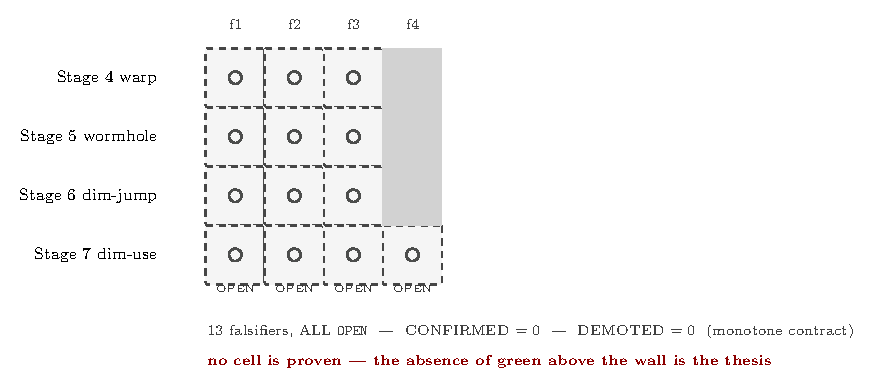
\includegraphics[width=0.88\linewidth]{figures/fig06_falsifier_matrix.pdf}
\caption{The Stage-4--7 falsifier status matrix: all 13 cells are
\texttt{OPEN} (open grey circles), \texttt{CONFIRMED}$=0$ and
\texttt{DEMOTED}$=0$. The four rows are the four upper-ladder stages
(warp/wormhole/dim-jump/dim-use); columns are the per-stage falsifier
indices. \emph{No cell is green} --- that absence is the thesis. A cell
moves only on an empirical measurement (the measurand named in
Table~\ref{tab:s47}), never by the act of integration. The monotone
contract permits only $\texttt{OPEN}\to\texttt{CONFIRMED}$ or
$\texttt{OPEN}\to\texttt{DEMOTED}$; silent retraction is forbidden.}
\label{fig:s47-matrix}
\end{figure}

% -------------------------------------------------------------------------
\subsection{The four per-stage metric folds (lattice arithmetic only)}
\label{app:s47-folds}

Each upper rung carries an $n\!=\!6$ lattice projection of a known GR /
string metric. The integers are exact; the physics is not.

\paragraph{Stage-4 warp (Alcubierre).}
$ds^2=-c^2dt^2+(dx-v_s f(r_s)\,dt)^2+dy^2+dz^2$, with the lattice fixing
the wall thickness, York asymmetry, and Van~Den~Broeck reduction:
\begin{equation}
\delta=\tfrac1{\sigma(6)}\,\ell_{\text{Pl}}=\tfrac1{12}\ell_{\text{Pl}},
\quad
\frac{\theta_{\text{fwd}}}{\theta_{\text{rear}}}=\sigma(6)=12,
\quad
E_{\text{neg}}^{\text{VDB}}=\frac{E_{\text{neg}}}{\sigma^2}=\frac{E_{\text{neg}}}{144}.
\label{eq:s47-warp}
\end{equation}
\paragraph{Stage-5 wormhole (Morris--Thorne).}
$ds^2=-e^{2\Phi(r)}c^2dt^2+\frac{dr^2}{1-b(r)/r}+r^2d\Omega^2$, throat
$b(b_0)=b_0$, flare-out $b'(b_0)<1$:
\begin{equation}
b_0=\ell_{\text{Pl}}\,\sigma(6)=12\,\ell_{\text{Pl}},
\quad
\Delta\tau_{\text{trav}}\ge\bigl(\sigma(6)-\varphi(6)\bigr)\tfrac{b_0}{c}=\tfrac{10\,b_0}{c},
\quad
\text{ANEC factor}=\tfrac1{\tau(6)}=\tfrac14.
\label{eq:s47-worm}
\end{equation}
Linear-perturbation stability requires at least $\varphi(6)=2$
independent NEC-violating channels (else quantum-interest collapse).
\paragraph{Stage-6 dim-jump (Kaluza--Klein ladder).}
$4\text{D}\to6\text{D}\to10\text{D}\to11\text{D}\to24\text{D}\to26\text{D}$
keyed to the divisor functions ($\tau{=}4$, $n{=}6$, $\sigma{-}\varphi{=}10$,
$\sigma{-}\mu{=}11$, $J_2{=}24$, $J_2{+}\varphi{=}26$):
\begin{equation}
R_c=\ell_{\text{Pl}}\,\sigma(6)^{n/\varphi}=\ell_{\text{Pl}}\,12^3=1728\,\ell_{\text{Pl}},
\quad
m_{\text{KK}}=\frac{n\hbar}{R_c c},
\quad
E_{\text{fold}}=\frac{M_{\text{Pl}}c^2}{(\sigma-\varphi)^d}=\frac{M_{\text{Pl}}c^2}{10^d}.
\label{eq:s47-dim}
\end{equation}
\paragraph{Stage-7 dim-use (composite $\tau{=}4$ cycle).}
The composite of warp and dim-jump (UNPROVEN$^2$):
\begin{equation}
\sigma\!\cdot\!\varphi=n\!\cdot\!\tau=J_2=24,
\qquad
(\sigma-\varphi)^2=(12-2)^2=100\,c
\quad(\text{effective composite speed}),
\label{eq:s47-use}
\end{equation}
a $\tau{=}4$ stage cycle (fold $\to$ warp-accelerate $\to$ cruise $\to$
dim-jump) whose closure is itself unproven.

% -------------------------------------------------------------------------
\subsection{Arithmetic closure $\ne$ empirical truth}
\label{app:s47-honest}

The single most important statement of this appendix: every integer in
Eqs.~\eqref{eq:s47-warp}--\eqref{eq:s47-use} is a verifiable
$\Pi^0_1$-arithmetical identity (checkable in one line via
\verb|UFO/verify/lattice_check.hexa| and the \verb|numerics_*.hexa|
parity scripts). \textbf{The verifiability of the integers transfers
\emph{no} truth to the physics they index.} $\sigma\!\cdot\!\tau=48$
closes as an integer product; whether a $48$-T field, a $12\,\ell_{\text{Pl}}$
throat, or a $100c$ composite speed \emph{exists} is an entirely separate,
academically unproven question. The proper epistemic form for an unproven
speculative claim is exactly this preregister: name the measurement that
would break it, and leave it \texttt{OPEN} until the measurement is made.
This is not an impossibility verdict (@D~d2): F-WARP-1 names bench-scale
Casimir negative-energy + QI-bound extrapolation, F-DIM-1 names the LHC
14\,TeV KK hunt, F-DIM-2 names sub-mm Eot--Wash torsion-balance gravity
--- concrete empirical breakthrough paths, all currently \texttt{OPEN}.

% -------------------------------------------------------------------------
\subsection{The monotone state contract}
\label{app:s47-monotone}

The falsifier state set is $\{\texttt{OPEN},\texttt{CONFIRMED},
\texttt{DEMOTED}\}$ with monotone transitions only:
\[
\texttt{OPEN}\longrightarrow\texttt{CONFIRMED}
\quad(\text{empirically confirmed }\Rightarrow\text{ lattice claim DEMOTED}),
\qquad
\texttt{OPEN}\longrightarrow\texttt{DEMOTED}
\quad(\text{empirical progress confirms a prediction}).
\]
Silent retraction is forbidden. At v1.0 all 13 are \texttt{OPEN}, so the
upper ladder contributes \emph{zero} proven content and the integration
bit cannot move from \texttt{absorbed=false} on its account. Crucially,
\tierWhite\ \textbf{never graduates to \tierGreen\ by sharing a table with
\tierGreen} (Stages~1--3); only an empirical observation can change a
falsifier's state.
